\documentclass{article}
\usepackage[T1]{fontenc}
\usepackage[utf8]{inputenc}
\usepackage[portuguese]{babel}

\title{Lista 3 \\
\large Introdução à Análise Numérica \\
Interpolação}
\author{Lucas Emanuel Resck Domingues}
\date{Outubro de 2020}

\usepackage{natbib}
\usepackage{graphicx}
\usepackage{amsmath}
\usepackage{listings}
\usepackage{multirow}
\usepackage{hyperref}
\usepackage{amsfonts}

\lstset{columns=fullflexible}

%Hyperlinks
\usepackage{hyperref}
\hypersetup{
    colorlinks=true,
    allcolors=,  % Nothing change colors
    urlcolor=blue  % URL changes color
}

\begin{document}

    \maketitle

    \begin{enumerate}
        \item[2.] Vamos utilizar o método das diferenças de Newton,
            encontrar os coeficientes $c_n$ e finalmente encontrar $P(k)$.

            $P$ é um polinômio de grau $n$, e sabemos que ele passa
            pelos pontos

            $$(1, -1), (2, -2), \cdots, (n, -n), (0, (-1)^n)$$

            sendo o último ponto justificado por $P(0) = (-1)^n$
            (termo independente).
            Então o polinômio escrito na forma do método das diferenças fica

            \begin{align*}
                P(x) &= c_0 + c_1 (x - x_1) + \cdots + c_n (x - x_1)\cdots(x - x_n) \\
                &= c_0 + c_1 (x - 1) + \cdots + c_n (x - 1)\cdots(x - n) \\
            \end{align*}

            A Tabela \ref{tab:diff} mostra o cálculo dos coeficientes $c_i$
            pelo método das diferenças de Newton.

            % https://www.tablesgenerator.com/
            
            \begin{table}[!h]
                \centering
                \begin{tabular}{c|c|c|c|c|l}
                    x &
                    $y=\Delta^1$ &
                    $\Delta^2$ &
                    $\Delta^3$ &
                    $\Delta^4$ &
                    \multirow{18}{*}{$\cdots$} \\ \cline{1-5}
                    \multirow{2}{*}{1} &
                    \multirow{2}{*}{$\mathbf{-1}$} &
                    &
                    &
                    &
                    \\
                    &
                    &
                    \multirow{2}{*}{$\mathbf{-1}$} &
                    &
                    &
                    \\
                    \multirow{2}{*}{2} &
                    \multirow{2}{*}{$-2$} &
                    &
                    \multirow{2}{*}{$\mathbf{0}$} &
                    &
                    \\
                    &
                    &
                    \multirow{2}{*}{$-1$} &
                    &
                    \multirow{2}{*}{$\mathbf{0}$} &
                    \\
                    \multirow{2}{*}{3} &
                    \multirow{2}{*}{$-3$} &
                    &
                    \multirow{2}{*}{0} &
                    &
                    \\
                    &
                    &
                    \multirow{2}{*}{$-1$} &
                    &
                    \multirow{2}{*}{0} &
                    \\
                    \multirow{2}{*}{4} &
                    \multirow{2}{*}{$-4$} &
                    &
                    \multirow{2}{*}{0} &
                    &
                    \\
                    &
                    &
                    \multirow{2}{*}{$-1$} &
                    &
                    \multirow{2}{*}{0} &
                    \\
                    \multirow{2}{*}{5} &
                    \multirow{2}{*}{$-5$} &
                    &
                    \multirow{2}{*}{0} &
                    &
                    \\
                    &
                    &
                    \multirow{3}{*}{$\vdots$} &
                    &
                    \multirow{3}{*}{$\vdots$} &
                    \\
                    $\vdots$ &
                    $\vdots$ &
                    &
                    $\vdots$ &
                    &
                    \\
                    \multirow{2}{*}{$n-1$} &
                    \multirow{2}{*}{$-(n-1)$} &
                    &
                    \multirow{2}{*}{0} &
                    &
                    \\
                    &
                    &
                    \multirow{2}{*}{$-1$} &
                    &
                    \multirow{2}{*}{$C(n)$} &
                    \\
                    \multirow{2}{*}{n} &
                    \multirow{2}{*}{$-n$} &
                    &
                    \multirow{2}{*}{$B(n)$} &
                    &
                    \\
                    &
                    &
                    \multirow{2}{*}{$A(n)$} &
                    &
                    &
                    \\
                    \multirow{2}{*}{0} &
                    \multirow{2}{*}{$(-1)^n$} &
                    &
                    &
                    &
                    \\
                    &
                    &
                    &
                    &
                    &
                
                \end{tabular}
                \caption{Método das diferenças de Newton para o polinômio $P$.
                Os números em negrito são os coeficientes $c_i$.
                Os números $A(n), \cdots$ são funções de $n$, não necessariamente $0$.}
                \label{tab:diff}
            \end{table}

            Dessa forma, nós concluímos que $c_0 = c_1 = -1$ e que
            $c_2 = \cdots = c_{n-1} = 0$.
            Apenas nos resta encontrar $c_n$, que, seguindo a tabela,
            será uma função de $n$. Até agora, temos
            
            $$P(x) = -1 -1(x-1) + c_n(x-1)\cdots(x-n)$$

            Sabendo que $P(0) = (-1)^n$, vemos que

            \begin{align*}
                P(0) &= (-1)^n \\
                c_n(-1)\cdots(-n) &= (-1)^n \\
                c_n(-1)^n n! &= (-1)^n \\
                c_n &= \dfrac{1}{n!} \\
            \end{align*}

            Tendo todos os coeficientes, podemos calcular $P(k)$, $k$ natural e maior que $n$:

            \begin{align*}
                P(k) &= -1-1(k-1)+\dfrac{1}{n!}(k-1)\cdots(k-n) \\
                &= -k + \dfrac{(k-1)!}{n!(k-1-n)!} \\
                &= {k-1\choose n} - k
            \end{align*}

        \pagebreak

        \item[8.] Vamos montar os polinômios interpoladores $p_{k-2}$ e $p_{k-1}$ de graus
            $k-2$ e $k-1$, respectivamente, através do método das diferenças de Newton.
            Depois vamos encontrar o coeficiente $c_{k-1}$, que corresponde
            a $\Delta[x_1, \cdots, x_k]$. Ao final, vamos calcular o limite pedido.
            
            Seja o polinômio interpolador $p_{k-2}$ de $f$ com os pontos $\{x_1, \cdots, x_{k-1}\}$ através dos métodos das diferenças de Newton:
            
            $$p_{k-2}(x) = c_0 + \cdots + c_{k-2} (x - x_1)\cdots(x - x_{k-2})$$

            Uma das principais características do método de Newton é que podemos ``reutilizar'' o polinômio
            ao adicionar mais pontos. Se quisermos interpolar $\{x_1, \cdots, x_k\}$, basta fazermos
            
            $$p_{k-1}(x) = c_0 + \cdots + c_{k-2} (x - x_1)\cdots(x - x_{k-2}) + c_{k-1} (x - x_1)\cdots(x - x_{k-1})$$

            Observe que $c_{k-1}$ corresponde a $\Delta[x_1, \cdots, x_k]$, que é o que queremos. Segue:

            \begin{align}
                p_{k-1}(x) - p_{k-2}(x) &= c_{k-1} (x - x_1)\cdots(x - x_{k-1}) \nonumber \\
                (f(x) - p_{k-2}(x)) - (f(x) - p_{k-1}(x)) & = c_{k-1} (x - x_1)\cdots(x - x_{k-1}) \label{eq:first}
            \end{align}

            Seja $A = [\min\{x_1, \cdots, x_k\}, \max\{x_1, \cdots, x_k\}]$.
            Por conveniência, assumindo que $\{x_1, \cdots, x_k\}$ são diferentes
            e sabendo que $f(x) = \sin(cx + d)$ é de classe $C^\infty$ no intervalo $A$,
            sabemos, por teorema, que, para cada $x \in A$,
            existem $\alpha_x, \beta_x$
            tais que

            $$f(x) - p_{k-2}(x) = \dfrac{f^{(k-1)}(\alpha_x)}{(k-1)!}(x-x_1)\cdots(x-x_{k-1})$$
            $$f(x) - p_{k-1}(x) = \dfrac{f^{(k)}(\beta_x)}{k!}(x-x_1)\cdots(x-x_k)$$

            Então, se avaliarmos essas funções em $x_k$ e substituirmos na Equação \ref{eq:first}, obtemos

            \begin{align*}
                \dfrac{f^{(k-1)}(\alpha_{x_k})}{(k-1)!}(x_k-x_1)\cdots(x_k-x_{k-1}) &= c_{k-1} (x_k - x_1)\cdots(x_k - x_{k-1}) \\
                \dfrac{f^{(k-1)}(\alpha_{x_k})}{(k-1)!} &= c_{k-1}
            \end{align*}

            Segue portanto:

            \begin{align*}
                |c_{k-1}| &= \left|\dfrac{f^{(k-1)}(\alpha_{x_k})}{(k-1)!}\right| \\
                &= \dfrac{|c^{k-1} \sin(c \alpha_{x_k}+d)|}{(k-1)!} \textrm{ ou } \dfrac{|c^{k-1} \cos(c \alpha_{x_k}+d)|}{(k-1)!} \\
                &\le \dfrac{|c|^{k-1}}{(k-1)!}
            \end{align*}

            Basta agora mostrar que isso tende a zero quando k tende ao infinito.
            Ou seja, vamos mostrar que, se $a \ge 0$,

            $$\lim_{k \to \infty} \dfrac{a^k}{k!} = 0$$

            Seja a sequência $y_k = \dfrac{a^k}{k!}$. Considere o termo $y_{2a+1}$. Então:

            $$y_{2a+1} = \dfrac{a^{2a+1}}{(2a+1)!} = \dfrac{a^{2a}}{(2a)!}\dfrac{a}{2a + 1} < \dfrac{a^{2a}}{(2a)!}\dfrac{1}{2} = \dfrac{1}{2} y_{2a}$$

            Concluímos que, para $k \in \mathbb{N}^*$, $y_{2a+k} < \left(\dfrac{1}{2}\right)^k y_{2a}$. Logo:

            $$\lim_{k \to \infty} \dfrac{a^k}{k!} = \lim_{k \to \infty} y_k = \lim_{k \to \infty} y_{2a+k} \le \lim_{k \to \infty} \left(\dfrac{1}{2}\right)^k y_{2a} = 0$$

            Portanto, $c_{k-1} \to 0$, ou seja, $\Delta[x_1, \cdots, x_k] \to 0$

        \pagebreak

        \item[12.]
            \begin{enumerate}
                \item Sejam os pontos $(x_0, y_0), \cdots, (x_n, y_n)$,
                    enumerados a partir do zero por conveniência.
                    Ou seja, $n + 1$ pontos.
                    Os pontos guia são $(\hat{x}_0, \hat{y}_0)$, $(\hat{x}_n, \hat{y}_n)$
                    Vamos asssumir intervalos de comprimento $h_i = 1/n$,
                    isso é, teremos $t_0 < \cdots < t_n$,
                    com $t_i = \dfrac{i}{n}$ (a conveniência).
                    Portanto, vamos interpolar os $n+1$ pontos
                    com a curva $\gamma(t) = (x(t), y(t))$, $t \in [0, 1]$.

                    Vamos interpolar cada intervalo $[t_i, t_{i+1}]$,
                    para $i=0,\cdots,n-1$, através de um polinômio de grau 3.
                    Vamos listar as condições que queremos para nossa curva $\gamma$:

                    \begin{itemize}
                        \item Passar pelos pontos: $\gamma(t_i) = (x(t_i), y(t_i)) = (x_i, y_i)$, $i = 0, \cdots, n$
                        \item Ancoragem 1: $\gamma'(0) = (x'(0), y'(0)) = k_0(\hat{x}_0 - x_0, \hat{y}_0 - y_0)$
                        \item Ancoragem 2: $\gamma'(1) = (x'(1), y'(1)) = k_1(\hat{x}_n - x_n, \hat{y}_n - y_n)$
                        \item Continuidade de $\gamma$ em $t_i$, $i = 1, \cdots, n-1$
                        \item Continuidade de $\gamma'$ em $t_i$, $i = 1, \cdots, n-1$
                        \item Continuidade de $\gamma''$ em $t_i$, $i = 1, \cdots, n-1$
                    \end{itemize}

                    Observe que nada impede de aplicarmos as condições de $\gamma$
                    separadamente para cada componente $x$ e $y$. Consideremos $x$.
                    Então, aplicando todas essas condições separadamente para $x$:

                    \begin{itemize}
                        \item Passar pelos pontos: $x(t_i) = x_i$, $i = 0, \cdots, n$
                        \item Ancoragem 1: $x'(0) = k_0(\hat{x}_0 - x_0)$
                        \item Ancoragem 2: $x'(1) = k_1(\hat{x}_n - x_n)$
                        \item Continuidade de $x$ em $t_i$, $i = 1, \cdots, n-1$
                        \item Continuidade de $x'$ em $t_i$, $i = 1, \cdots, n-1$
                        \item Continuidade de $x''$ em $t_i$, $i = 1, \cdots, n-1$
                    \end{itemize}

                    Ora, estamos pedindo uma interpolação por uma \textit{spline}
                    cúbica ancorada para $x$, afinal os valores de $t_i$ são crescentes.
                    Isso já foi estudado. Então sabemos que,
                    se $t \in [t_i, t_{i+1}]$,

                    \begin{align*}
                        x(t) &= \dfrac{M_i}{6h_i}(t_{i+1}-t)^3 + \dfrac{M_{i+1}}{6h_i}(t-t_i)^3 + c_1t+c_2 \\
                        &= \dfrac{nM_i}{6}(t_{i+1}-t)^3 + \dfrac{nM_{i+1}}{6}(t-t_i)^3 + c_1t+c_2 \\
                    \end{align*}

                    sendo

                    \begin{align*}
                        c_1 &= \dfrac{x_{i+1}-x_i}{h_i} -\dfrac{h_i}{6}(M_{i+1}-M_i) \\
                        &= n(x_{i+1}-x_i) -\dfrac{1}{6n}(M_{i+1}-M_i) \\
                    \end{align*}

                    \begin{align*}
                        c_2 &= x_i - \dfrac{M_i h_i^2}{6} - c_1 t_i \\
                        &= x_i - \dfrac{M_i}{6n^2} - c_1 t_i \\
                    \end{align*}
                    
                    Os valores de $M_i$, por sua vez, são encontrados através das equações

                    $$\dfrac{1}{6n}M_{i-1} + \dfrac{2}{3n}M_i + \dfrac{1}{6n}M_{i+1} = n(x_{i+1} - 2x_i + x_{i-1})$$

                    para $i = 1, \cdots, n-1$. Essas equações são encontradas aplicando as condições
                    dadas acima, com exceção das ancoragens. Como isso foi feito em sala,
                    é conveniente omitir essa dedução. Porém, essas equações são em quantidade
                    $n-1$, e temos $n+1$ variáveis $M_i$ para descobrir: $M_0, \cdots, M_n$.

                    Para resolver isso, podemos aplicar as condições de ancoragem em $t_0 = 0$ e $t_n = 1$.
                    Basta resolver $x'(0) = k_0(\hat{x}_0 - x_0)$. Vejamos. Para $t \in [0, 1/n]$, vale que:

                    $$x'(t) = -\dfrac{M_0}{2h_0}(t_1 - t)^2 + \dfrac{M_1}{2h_0}(t-t_0)^2 + \dfrac{x_1 - x_0}{h_0} - \dfrac{h_0}{6}(M_1 - M_0)$$

                    Então:

                    \begin{align*}
                        x'(0) &= k_0(\hat{x}_0 - x_0) \\
                        -\dfrac{M_0}{3n} + n(x_1 - x_0) - \dfrac{M_1}{6n} &= k_0(\hat{x}_0 - x_0) \\
                        \dfrac{1}{3n}M_0 + \dfrac{1}{6n}M_1 &= -k_0(\hat{x}_0 - x_0) + n(x_1 - x_0) \\
                    \end{align*}

                    De forma análoga:

                    $$\dfrac{1}{6n}M_{n-1} + \dfrac{1}{3n}M_n = k_1 (\hat{x}_n - x_n) - n(x_n - x_{n-1})$$

                    Encontramos as duas equações que estavam faltando. Sendo assim, podemos montar o seguinte
                    sistema de equações que deve ser resolvido:

                    $$Ax = b$$

                    sendo

                    $$A = \begin{bmatrix}
                        \dfrac{1}{3n} & \dfrac{1}{6n}  \\[6pt]
                        \dfrac{1}{6n} & \dfrac{2}{3n} & \dfrac{1}{6n}  \\[6pt]
                        & \dfrac{1}{6n} & \dfrac{2}{3n} & \dfrac{1}{6n}  \\[6pt]
                        & & & & \ddots \\[6pt]
                        & & & & & \dfrac{1}{6n} & \dfrac{2}{3n} & \dfrac{1}{6n}  \\[6pt]
                        & & & & & & \dfrac{1}{6n} & \dfrac{1}{3n}  \\[6pt]
                        \end{bmatrix}$$
                    $$x = \begin{bmatrix}
                            M_0 \\
                            \vdots \\
                            M_n
                        \end{bmatrix}$$
                    $$b = \begin{bmatrix}
                            -k_0(\hat{x}_0 - x_0) + n(x_1 - x_0) \\
                            n(x_{2} - 2x_1 + x_{0}) \\
                            \vdots \\
                            n(x_n - 2x_{n-1} + x_{n-2}) \\
                            k_1 (\hat{x}_n - x_n) - n(x_n - x_{n-1})
                        \end{bmatrix}$$

                    Ou seja, conseguindo todos os $M_i$, a partir de um algoritmo
                    de resolução de sistemas lineares (observe que o sistema
                    é diagonalmente dominante, perfeito para vários métodos estudados
                    em aula), calculamos $c_1$ e $c_2$ e podemos
                    expressar $x(t)$.

                    O processo para $y$ é totalmente análogo.

                    Ao final, temos $\gamma(t) = (x(t), y(t))$.

                \item O programa foi implementado em Matlab e pode ser conferido no Apêndice
                    \ref{appendix:splines}.
                    A utilização do programa se dá da seguinte forma:
                    vamos montar $k$ \textit{splines} cúblicas paramétricas, cada \textit{spline}
                    emendada à anterior. Cada \textit{spline} será composta de $n + 3$ pontos,
                    sendo $n + 1$ os pontos de interpolação $(x_0, y_0), \cdots, (x_n, y_n)$
                    e 2 pontos de ancoragem $(\hat{x}_0, \hat{y}_0), (\hat{x}_n, \hat{y}_n)$.
                    Iniciamos a função com o comando
                    
                    \begin{center}
                        \lstinline{interactive_spline(n, k, k_0, k_1)}
                    \end{center}

                    sendo $k_0$, $k_1$ relacionados à ancoragem, já vistos anteriormente.
                    Sendo assim, desenha-se os pontos, na ordem

                    $$(x_0, y_0), (\hat{x}_0, \hat{y}_0), (x_1, y_1), \cdots, (x_n, y_n), (\hat{x}_n, \hat{y}_n)$$

                    um total de $k$ vezes.

                    O programa lê os pontos selecionados e constrói, para cada intervalo $[t_i, t_{i+1}]$,
                    o polinômio interpolador, tanto para $x$ quanto para $y$.
                    O sistema de equações lineares é resolvido utilizando
                    o método de Seidel (já implementado em exercícios anteriores deste curso),
                    afinal a matriz é diagonalmente dominante.
                    Os dois polinômios resultantes em cada pequeno intervalo são calculados
                    e exibidos graficamente para vários
                    pontos desse pequeno intervalo, dando a ideia de continuidade.

                    As Figuras \ref{fig:abcde}, \ref{fig:t} e \ref{fig:5} mostram
                    exemplos do resultado da utilização do programa.

                    \begin{figure}[!h]
                        \centering
                        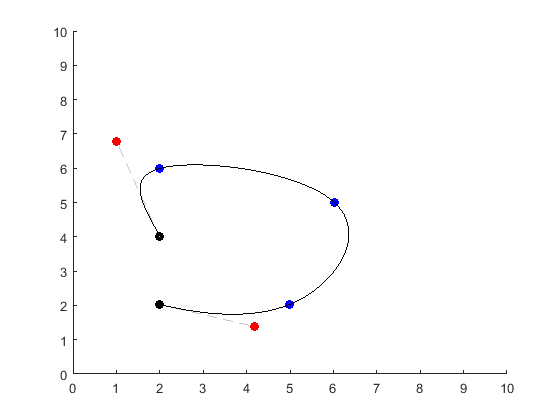
\includegraphics[width=0.8\textwidth]{images/abcde.png}
                        \caption{Interpolação por \textit{spline} cúbica paramétrica
                        para 5 pontos de interpolação e 2 pontos de ancoragem.}
                        \label{fig:abcde}
                    \end{figure}

                    \begin{figure}[!h]
                        \centering
                        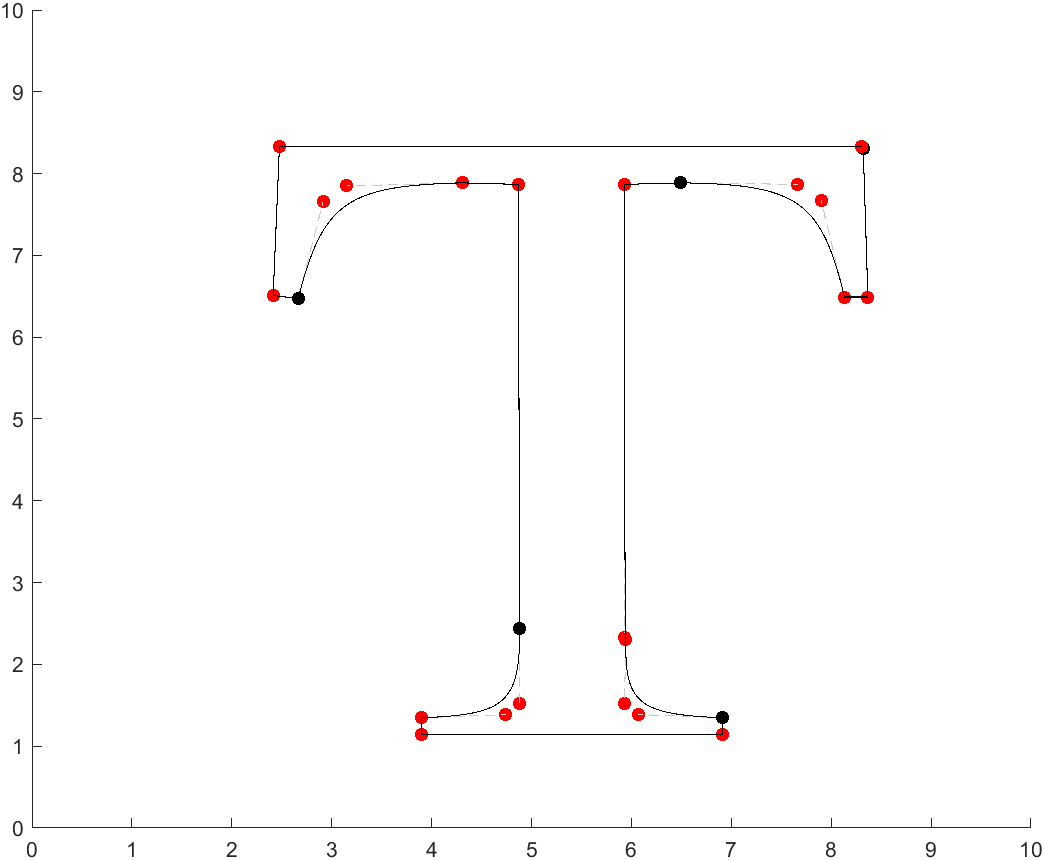
\includegraphics[width=0.8\textwidth]{images/t.png}
                        \caption{Interpolação por várias \textit{splines} cúbicas paramétricas
                        para 2 pontos de interpolação e 2 pontos de ancoragem.}
                        \label{fig:t}
                    \end{figure}

                    \begin{figure}[!h]
                        \centering
                        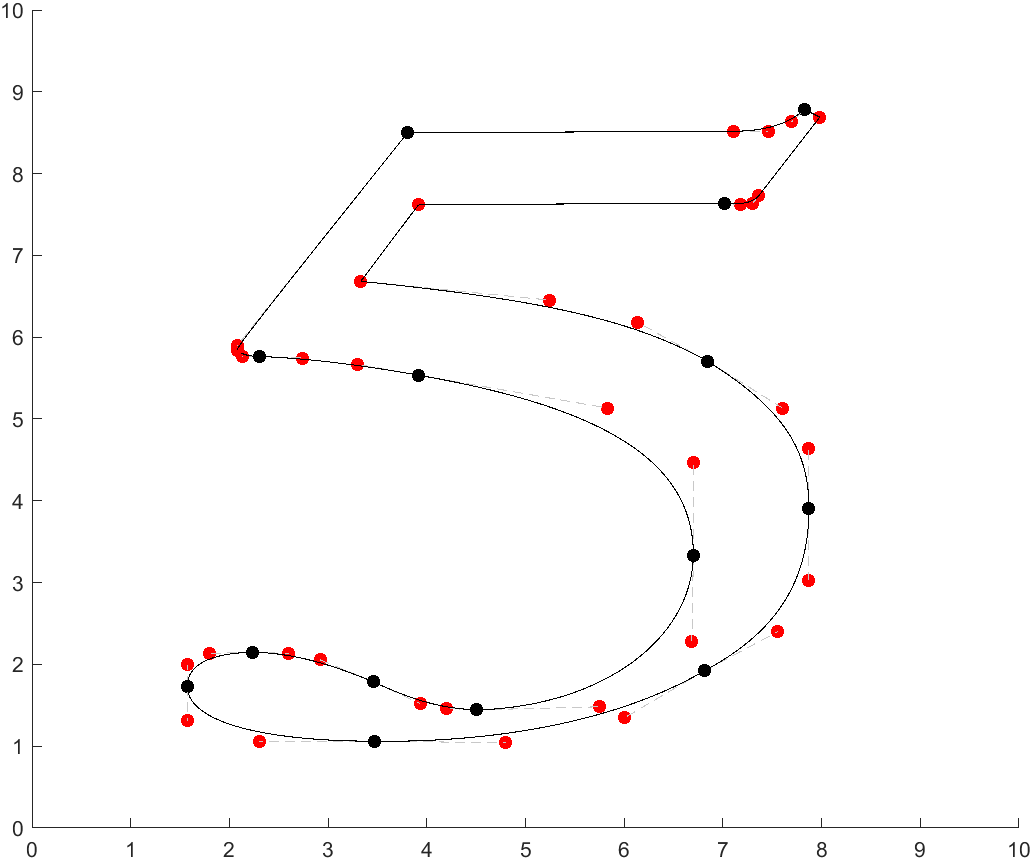
\includegraphics[width=0.8\textwidth]{images/5.png}
                        \caption{Interpolação por várias \textit{splines} cúbicas paramétricas
                        para 2 pontos de interpolação e 2 pontos de ancoragem.}
                        \label{fig:5}
                    \end{figure}
                                        
            \end{enumerate}

    \end{enumerate}

    \clearpage

    \appendix

    \section{Programa computacional para \textit{splines} interativos}
        \label{appendix:splines}

        Implementação do algoritmo em Matlab
        para construção de \textit{splines} cúbicos paramétricos
        interativos. O código também pode ser acessado
        \href{https://github.com/lucasresck/introduction-to-numerical-analysis/blob/master/list_3/interactive_spline.m}{no GitHub}.

        \begin{lstlisting}[language=Matlab]
function interactive_spline(n, k, k_0, k_1)
    clf;
    axis([0, 10, 0, 10]);
    hold on;
    [x_click, y_click] = ginput(1);
    x = [x_click];
    y = [y_click];
    plot(x, y, 'o', ...
        'MarkerEdgeColor', 'k', ...
        'MarkerFaceColor', 'k');
    for j = 1:k
        for i = 1:n+2
            [x_click, y_click] = ginput(1);
            x = [x; x_click];
            y = [y; y_click];
            if i == 1 || i == n+2
                plot(x_click, y_click, 'o', ...
                'MarkerEdgeColor', 'r', ...
                'MarkerFaceColor', 'r');
                plot(x(end-1:end), y(end-1:end), '--', ...
                    'Color', [200, 200, 200]/255);
            else
                if i == n+1
                    plot(x_click, y_click, 'o', ...
                    'MarkerEdgeColor', 'k', ...
                    'MarkerFaceColor', 'k');
                else
                    plot(x_click, y_click, 'o', ...
                    'MarkerEdgeColor', 'b', ...
                    'MarkerFaceColor', 'b');
                end
            end
        end
        parametric_cubic_spline(x, y, k_0, k_1);
        x = [x(end-1)];
        y = [y(end-1)];
    end
    hold off;
end

function parametric_cubic_spline(x, y, k_0, k_1)
    x_t = anchored_cubic_spline(x, k_0, k_1);
    y_t = anchored_cubic_spline(y, k_0, k_1);
    plot(x_t, y_t, '-k');
end

function x_t = anchored_cubic_spline(x, k_0, k_1)
    x_hat_0 = x(2);
    x_hat_n = x(end);
    x(end) = [];
    x(2) = [];
    [n, ~] = size(x);
    n = n-1;
    h = 1/n;
    A = zeros(n+1, n+1);
    b = zeros(n+1, 1);
    for i=0:n
        if i == 0
            j = i+1;
            A(j, j) = 1/(3*n);
            A(j, j+1) = 1/(6*n);
            b(j) = -k_0*(x_hat_0 - x(j)) + n*(x(j+1) - x(j));
        else
            if i == n
                j = i+1;
                A(j, j-1) = 1/(6*n);
                A(j, j) = 1/(3*n);
                b(j) = k_1*(x_hat_n - x(j)) - n*(x(j) - x(j-1));
            else
                j = i+1;
                A(j, j-1) = 1/(6*n);
                A(j, j) = 2/(3*n);
                A(j, j+1) = 1/(6*n);
                b(j) = n*(x(j+1) - 2*x(j) + x(j-1));
            end
        end
        
    end
    M = seidel(A, b, 10^-6);
    x_t = [];
    for i=0:(n-1)
        p = interpolator(M(i+1), M(i+2), i/n, (i+1)/n, x(i+1), x(i+2), n);
        x_t = [x_t, p(i/n:0.01:(i+1)/n)];
    end
end

function x = seidel(A, b, eps)
    [m, ~] = size(A);
    x = zeros(m, 1);
    err = 1;
    x_old = x;
    while err > eps
        for i=1:m
            x(i) = A(i, 1:(i-1))*x(1:(i-1)) + A(i, (i+1):m)*x((i+1):m);
            x(i) = -x(i);
            x(i) = x(i) + b(i);
            x(i) = x(i)/A(i, i);
        end
        err = norm(x - x_old, 'inf')/norm(x_old, 'inf');
        x_old = x;
    end
end

function x_t = interpolator(M_i, M_ip, t_i, t_ip, x_i, x_ip, n)
    c_1 = (x_ip-x_i)*n - (M_ip - M_i)/(6*n);
    c_2 = x_i - M_i/(6*n^2) - c_1*t_i;
    syms x_t(t);
    x_t(t) = n*M_i/6*(t_ip-t)^3 + n*M_ip/6*(t-t_i)^3 + c_1*t + c_2;
end
        \end{lstlisting}
\end{document}
